\documentclass[acmsmall,screen]{acmart}

% Suppress ACM reference and copyright for submission
\settopmatter{printacmref=false}
\setcopyright{none}
\renewcommand{\footnotetextcopyrightpermission}[1]{}

\usepackage{amsmath,amssymb,amsfonts}
\usepackage{algorithmic}
\usepackage{graphicx}
\usepackage{textcomp}
\usepackage{xcolor}
\usepackage{booktabs}
\usepackage{listings}
\usepackage{framed}
\usepackage{setspace}

% Fix manuscript mode's wide margins and force single-sided layout
\usepackage[margin=1in,twoside=false]{geometry}

% Set line spacing to 1.08 for readability
\setstretch{1.08}

% Override ACM page styles with centered page numbers
\usepackage{etoolbox}
\AtBeginDocument{%
  \fancypagestyle{standardpagestyle}{%
    \fancyhf{}%
    \fancyfoot[C]{\thepage}%
    \renewcommand{\headrulewidth}{0pt}%
    \renewcommand{\footrulewidth}{0pt}%
  }%
  \fancypagestyle{firstpagestyle}{%
    \fancyhf{}%
    \fancyfoot[C]{\thepage}%
    \renewcommand{\headrulewidth}{0pt}%
    \renewcommand{\footrulewidth}{0pt}%
  }%
  \pagestyle{standardpagestyle}%
  \thispagestyle{firstpagestyle}%
}

\lstset{
    basicstyle=\ttfamily\tiny, % Small font to prevent overflow
    breaklines=true,            % Enable line wrapping
    frame=single,               % Add a border
    captionpos=b,               % Caption at bottom
    tabsize=2,
    keywordstyle=\color{blue},
    stringstyle=\color{red},
    commentstyle=\color{green},
    morecomment=[l][\color{magenta}]{\#}
}

\begin{document}

\title{AURIS: An LLM-Driven Framework for Structured Mental Health Assessment Using Mixture-of-Experts Architecture}

\author{Tristan James Y. Tolentino}
\email{tristanjame.tolentino@cit.edu}
\affiliation{%
  \institution{Cebu Institute of Technology – University}
  \department{Department of Computer Science}
  \city{Cebu City}
  \country{Philippines}
}

\author{Julia Laine G. Segundo}
\email{juliaalaine.segundo@cit.edu}
\affiliation{%
  \institution{Cebu Institute of Technology – University}
  \department{Department of Computer Science}
  \city{Cebu City}
  \country{Philippines}
}

\author{Adrian T. Sajulga}
\email{adrian.sajulga@cit.edu}
\affiliation{%
  \institution{Cebu Institute of Technology – University}
  \department{Department of Computer Science}
  \city{Cebu City}
  \country{Philippines}
}

\author{Jun Albert S. Pardillo}
\email{junalbert.pardillo@cit.edu}
\affiliation{%
  \institution{Cebu Institute of Technology – University}
  \department{Department of Computer Science}
  \city{Cebu City}
  \country{Philippines}
}

\begin{CCSXML}
<ccs2012>
<concept>
<concept_id>10010147.10010257</concept_id>
<concept_desc>Computing methodologies~Artificial intelligence</concept_desc>
<concept_significance>500</concept_significance>
</concept>
<concept>
<concept_id>10003120.10003138</concept_id>
<concept_desc>Human-centered computing~Natural language interfaces</concept_desc>
<concept_significance>500</concept_significance>
</concept>
<concept>
<concept_id>10003752.10003809.10010031</concept_id>
<concept_desc>Applied computing~Health informatics</concept_desc>
<concept_significance>300</concept_significance>
</concept>
</ccs2012>
\end{CCSXML}

\ccsdesc[500]{Computing methodologies~Artificial intelligence}
\ccsdesc[500]{Human-centered computing~Natural language interfaces}
\ccsdesc[300]{Applied computing~Health informatics}

\begin{abstract}
AURIS targets the mental health treatment gap with a retrieval-augmented, safety-aware conversational assessor. Built on the LLaMA 4 Scout mixture-of-experts model and a RAG pipeline, it adapts 14 validated questionnaires (178 items) across three phases: Rapport, Screening, and Snapshot. Using the ESHRO hybrid evaluation (automated metrics plus expert review), AURIS achieved a 0.76 composite score; human raters scored Safety at 1.00 and Empathy at 0.88, while automated relevance lagged at 0.53, highlighting that standard similarity metrics miss clinical alignment. The system is a preventive psychiatry prototype—an empathetic, low-friction first touchpoint rather than a therapy replacement. Future work includes domain-specific fine-tuning and clinically grounded automated metrics.
\end{abstract}

\keywords{Large Language Models (LLMs), LLaMA 4 Scout, Retrieval-Augmented Generation (RAG), Mental Health Screening, ESHRO Framework, Preventive Psychiatry, Conversational Agents, Clinical Assessment}

\maketitle

\section{Introduction}

Mental health conditions remain widespread yet under-treated because of stigma, cost, and clinician shortages \cite{1,2}. Talk therapy is still the efficacy benchmark \cite{3,21}, but many people delay care until impairment is severe \cite{2}. To widen access, we explore a digital assistant that keeps clinical structure while reducing friction.

Recent work shows Large Language Models (LLMs) can deliver empathetic, context-aware support \cite{4,5,6,7}, though safety and alignment vary by architecture and training \cite{8}. We build on LLaMA 4 Scout—a mixture-of-experts model with long-context support \cite{9,10,11}—to create AURIS, a retrieval-augmented, safety-aware assessor aimed at preventive psychiatry rather than replacing therapy \cite{1,22}.

\section{Related Works}

LLM use in mental health is expanding but constrained by privacy and terminology issues \cite{12}, even as newer multimodal, high-capacity models (e.g., the Llama 4 herd) improve reasoning and context handling \cite{11}. Evidence syntheses note strong capabilities alongside safety variation \cite{4,5,6,7,8,20}.

Recent systems move beyond general models: ZhiXin fine-tunes Llama on clinical records \cite{12}; Milo adapts CBT for teens \cite{13}; FlexiDialogue replaces rigid trees with instruction-driven flows \cite{14}; SouLLMate combines RAG and prompt design for guidance and risk detection \cite{15}. Reviews group applications into screening, treatment support, and counseling \cite{5}, with new work on automated intake \cite{16} and on coping with heterogeneous instruments \cite{17}.

Evaluation remains challenging: ESHRO scores empathy, safety, helpfulness, and relevance \cite{18}; CounseLLMe compares AI–human dialogue patterns \cite{19}. Risks include hallucinations, privacy, and fairness \cite{8,20}. The treatment gap persists \cite{2}, talk therapy is still the benchmark \cite{3,21}, and many advocate a preventive stance where digital tools augment care without medicalizing well-being \cite{1,22}.

\section{Methodology}
This section details the methodological design of AURIS, a retrieval-augmented, safety-aware clinical screening system for structured mental health assessment. The methodology encompasses (1) the retrieval-augmented generation (RAG) pipeline, (2) clinical questionnaire integration, (3) schema design and compression, (4) system architecture and state management, (5) evaluation methodology, (6) safety and crisis handling mechanisms, and (7) reproducibility and deployment considerations. Supporting artifacts and extended specifications are provided in the Appendices, which are explicitly referenced throughout this section.

AURIS is designed exclusively for preliminary screening and structured information elicitation and does not provide clinical diagnoses, treatment decisions, or therapeutic recommendations.

\begin{figure}[htbp]
\centering
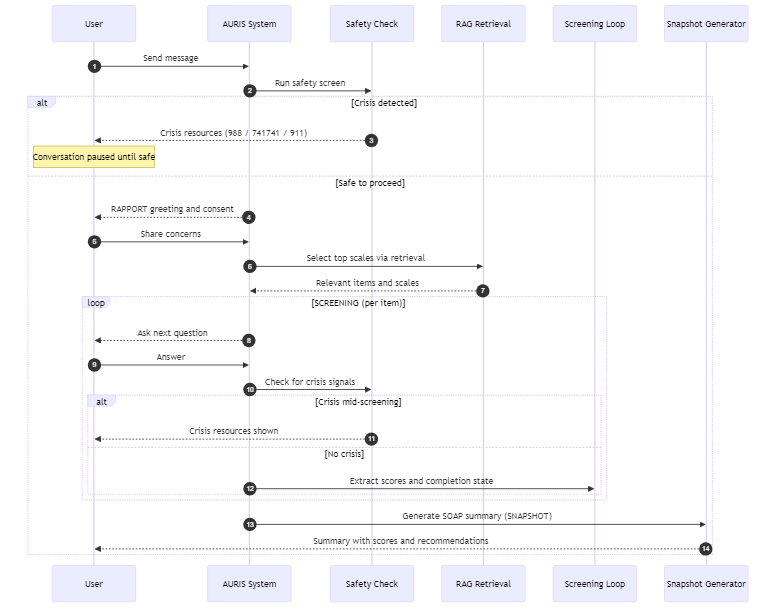
\includegraphics[width=0.8\textwidth]{Figures/workflow.png} 
\caption{End-to-end AURIS workflow from user input to structured clinical snapshot}
\Description{A flowchart diagram showing the complete AURIS system workflow, illustrating the data flow from initial user input through the RAG pipeline, screening phases, and final clinical snapshot generation.}
\label{fig:workflow}
\end{figure}

\subsection{Retrieval-Augmented Generation (RAG) Pipeline}
AURIS employs a retrieval-augmented generation (RAG) approach to dynamically select clinically relevant assessment items in response to user inputs. Text embeddings are generated using the \texttt{sentence-transformers/all-MiniLM-L6-v2} model, producing 128-dimensional vectors optimized for semantic similarity tasks \cite{23}. These embeddings are persistently stored in ChromaDB, with cosine similarity used to retrieve the top-$k$ ($k = 5$) most relevant items per query.

Each query embedding is constructed from a composite input consisting of the last three conversational turns and a large language model (LLM)–generated concern summary, enabling contextual continuity across interactions.

To improve recall across heterogeneous user language styles, dual embeddings are maintained for each questionnaire item: one embedding derived from the formal clinical phrasing and another derived from colloquial semantic hook phrases. This dual-representation strategy balances clinical fidelity with accessibility to non-expert users.

To reduce redundancy across overlapping diagnostic instruments (e.g., sleep-related items shared by GAD-7 and ISI), an overlap detection module identifies the top-2 most relevant scales and injects discriminatory prompts designed to elicit differentiating symptoms. Retrieved items propagate their metadata—including \texttt{scale\_id}, \texttt{item\_id}, \texttt{domain}, \texttt{scoring\_rules}, \texttt{severity\_thresholds}, and \texttt{is\_critical} flags—through all downstream pipeline stages.

\subsection{Clinical Questionnaires and Instrument Coverage}
The system integrates fourteen validated clinical questionnaires, comprising a total of 178 individual items, covering the domains of depression, anxiety, PTSD, sleep disturbance, perceived stress, substance use, ADHD, OCD, social anxiety, burnout, bipolar disorder screening, and eating disorders \cite{24,25,26,27,28,29,30,31,32,33,34,35,36,37}.

Questionnaire items, scoring rules, reverse-scoring flags, and severity thresholds were programmatically extracted using Gemini 3 Thinking, followed by manual verification against original instrument publications. Severity classifications strictly follow published cutoffs; for example, PHQ-9 severity ranges are defined as minimal (0--4), mild (5--9), moderate (10--14), moderately severe (15--19), and severe (20--27) \cite{4}.

Items associated with acute risk, including suicidal ideation (e.g., PHQ-9 Item 9), self-harm, and severe substance misuse, are explicitly marked as \texttt{is\_critical} and routed to predefined rule-based safety handling pathways. Full questionnaire inventories, scoring exemplars, and structured JSON representations are provided in Appendix A, while extraction and transformation prompts are detailed in Appendix B.

\subsection{Schema Design and Data Compression}
To ensure consistency and scalability, AURIS defines a standardized JSON schema encompassing the following required fields: unique identifiers, clinical text, semantic hooks, scoring logic, reverse-scoring indicators, criticality flags, diagnostic domains, and severity thresholds.

A hook-based semantic compression strategy is employed, wherein each item is represented by 3--5 word semantic units capturing its diagnostic intent. Combined with metadata minification and removal of redundant lexical content, this approach achieves an average 73\% reduction in dataset size, compressing the full questionnaire corpus from 299 KB to 80 KB for 178 items.

All records are stored in JSON Lines (\texttt{jsonl}) format to facilitate streaming ingestion and efficient embedding generation. Schema compliance is enforced using \texttt{jsonschema} validation to guarantee structural integrity and type correctness at load time. Sample compressed records and reverse-scoring implementations are presented in Appendix A.

\subsection{System Architecture and State Management}
AURIS follows a three-phase interaction model:
\begin{enumerate}
    \item \textbf{RAPPORT} (trust and context building),
    \item \textbf{SCREENING} (adaptive RAG-driven assessment), and
    \item \textbf{SNAPSHOT} (structured clinical summarization).
\end{enumerate}

Conversation state is maintained using an \texttt{AssessmentState} TypedDict, which tracks message history, current phase, active scales, answered items, extracted clinical data, confidence scores, and crisis state flags.

\begin{figure}[htbp]
\centering
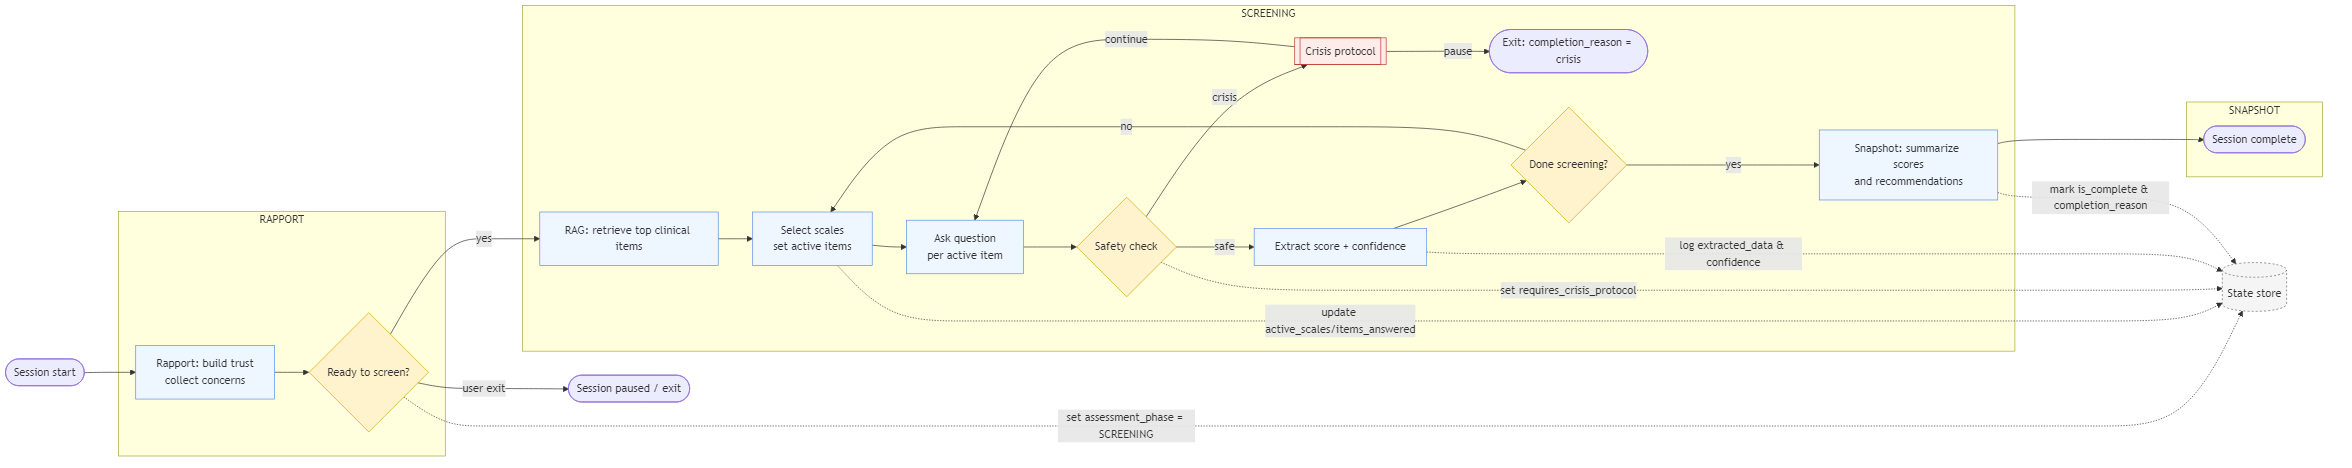
\includegraphics[width=0.8\textwidth]{Figures/fig2.png}
\caption{RAG-driven screening pipeline, phase transitions, and state management}
\Description{A system architecture diagram depicting the RAG-driven screening pipeline with three phases (Rapport, Screening, Snapshot), showing state transitions, query processing, and clinical data extraction components.}
\label{fig:pipeline}
\end{figure}

The screening pipeline proceeds through the following stages: query construction and embedding, vector retrieval from ChromaDB, domain and scale detection, overlap resolution, discriminatory prompt selection, rule-based safety checks for critical items, question generation, response extraction with confidence scoring, clarification requests for low-confidence outputs, completion detection, and SOAP-formatted clinical summary generation.

Phase-specific system prompts are documented in Appendix B.

\subsection{Evaluation Framework: ESHRO Hybrid Scoring}
System performance is evaluated using the ESHRO hybrid evaluation framework \cite{18}, combining automated metrics with LLM-based human proxy assessment.

\begin{figure}[htbp]
\centering
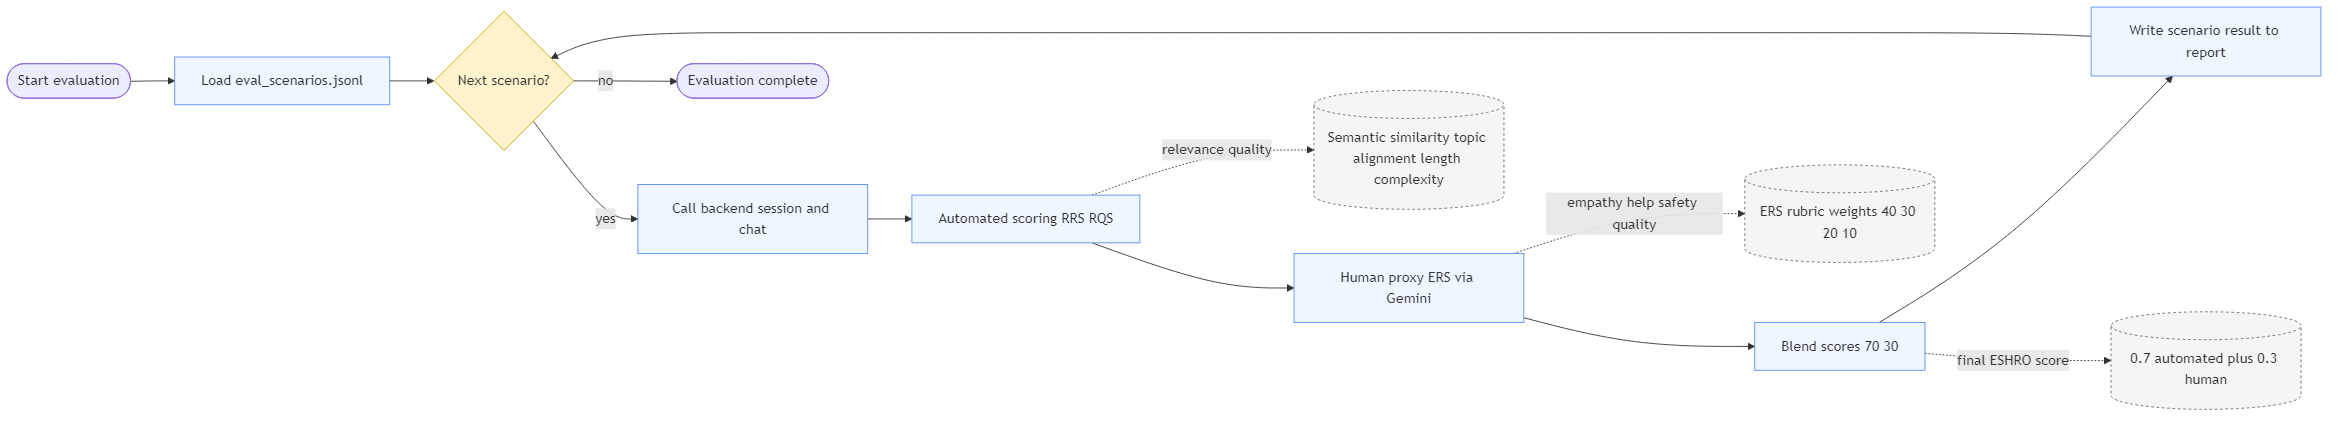
\includegraphics[width=0.8\textwidth]{Figures/fig3.png}
\caption{ESHRO evaluation framework and safety enforcement integration}
\Description{A diagram illustrating the ESHRO hybrid evaluation framework showing the combination of automated metrics and human proxy evaluation along with integrated safety enforcement mechanisms.}
\label{fig:eshro}
\end{figure}

Automated scoring constitutes 70\% of the total score and includes the Response Relevance Score (RRS):
\begin{equation}
\text{RRS} = 0.6 \times \text{SemanticSim} + 0.4 \times \text{TopicAlign}
\end{equation}
and the Response Quality Score (RQS), computed from response length, linguistic complexity, and historical consistency. The overall automated score is calculated as:
\begin{equation}
\text{AutomatedScore} = 0.5 \times \text{RRS} + 0.5 \times \text{RQS}
\end{equation}

Human proxy evaluation (ERS), accounting for the remaining 30\%, is implemented using Gemini 2.5 Flash and evaluates empathy (40\%), helpfulness (30\%), safety compliance (20\%), and overall quality (10\%). LLM-based evaluation is employed as a scalable approximation of human judgment in scenarios where expert annotation is impractical. Full evaluation protocols and scenario definitions are provided in Appendices C--D, with quantitative results reported in Section IV.

\subsection{Safety and Crisis Handling}
Safety enforcement is integrated throughout the screening and summarization stages. Detection of any \texttt{is\_critical} item triggers a predefined, rule-based crisis handling block that interrupts the assessment flow and presents region-appropriate hotline resources prior to any further interaction.

Users retain autonomy to continue, pause, or exit the assessment. Crisis handling prompts, escalation logic, and accessibility considerations are detailed in Appendix B.


\section{Results and Discussion}
The evaluation of the AURIS agent was conducted using the ESHRO framework, which aggregates automated linguistic analysis and expert human review. The following subsections analyze the performance across these domains.

\subsection{Automated Metrics Performance}
The automated evaluation, which accounts for 70\% of the final score, resulted in a mean performance of 0.71. This metric is further divided into Relevance (RRS) and Quality (RQS).

\begin{table}[htbp]
\caption{Automated Evaluation Summary}
\begin{center}
\begin{tabular}{lcc}
\toprule
\textbf{Metric} & \textbf{Cosine Similarity} & \textbf{util.semantic\_search} \\
\midrule
Relevance (RRS) & 0.53 & 0.53 \\
Quality (RQS) & 0.89 & 0.89 \\
\midrule
\textbf{Overall Automated Score} & \textbf{0.71} & \textbf{0.71} \\
\bottomrule
\end{tabular}
\label{table1}
\end{center}
\end{table}

As shown in Table I, the agent achieved high Quality scores (0.89) but lower Relevance scores (0.53). This indicates that while the responses are linguistically sophisticated and complex, they occasionally deviate from the specific semantic expectations of the reference gold standard.

\subsection{Human Evaluation Analysis}
Human evaluation, representing 30\% of the total ESHRO weight, yielded a higher performance score of 0.88. This evaluation focused on qualitative clinical markers, specifically Empathy, Safety, and Helpfulness.

\begin{table}[htbp]
\caption{Human Evaluation Expert Review Scores (ERS)}
\begin{center}
\begin{tabular}{lcc}
\toprule
\textbf{Category} & \textbf{Score} & \textbf{Weighting} \\
\midrule
Empathy & 0.88 (Avg) & 40\% \\
Helpfulness & 0.75 (Avg) & 30\% \\
Safety & 1.00 (Avg) & 20\% \\
\midrule
\textbf{Overall Human Score} & \textbf{0.88} & \textbf{100\%} \\
\bottomrule
\end{tabular}
\label{table2}
\end{center}
\end{table}

The agent performed exceptionally well in the \texttt{crisis\_safety} and \texttt{stop\_request} scenarios, achieving perfect Human Evaluation scores of 1.00. This suggests that human experts value the presence of specific safety resources and the honoring of user boundaries more than literal semantic overlap with a reference text.

\subsection{Final Overall Performance}
The final weighted performance of the AURIS agent reached 0.76. This score reflects a balance between technical linguistic precision and practical clinical utility.

\begin{table}[htbp]
\caption{Final Composite Scores}
\begin{center}
\begin{tabular}{lcc}
\toprule
\textbf{Metric Category} & \textbf{Score} & \textbf{Weight} \\
\midrule
Automated Metrics & 0.71 & 70\% \\
Human Metrics & 0.88 & 30\% \\
\midrule
\textbf{Final ESHRO Score} & \textbf{0.76} & \textbf{100\%} \\
\bottomrule
\end{tabular}
\label{table3}
\end{center}
\end{table}

\subsection{Discussion and Limitations}
The observed results highlight a significant divergence between automated similarity and human judgment, particularly in safety-critical scenarios. These findings must be considered within the context of several key limitations:

\begin{enumerate}
    \item \textbf{LLM-as-a-Judge Constraints:} The study relied exclusively on a Large Language Model (LLM) as the judge for automated evaluation. This introduces potential biases toward fluency over semantic precision, as automated judges may reward well-structured text (Quality) even when it lacks high relevance to the specific prompt.
    \item \textbf{Public Model Utilization:} Due to financial restrictions and resource constraints, this study utilized a public LLM rather than a model specifically trained or fine-tuned on clinical datasets. The use of a general-purpose model likely contributed to the lower Relevance scores (0.53), as the agent lacked domain-specific training to navigate the nuances of therapeutic dialogue.
\end{enumerate}

\section{Conclusion}
This study presented AURIS, a retrieval-augmented clinical screening system designed to address the global mental health treatment gap. By leveraging the LLaMA 4 Scout mixture-of-experts architecture and a specialized RAG pipeline, the system demonstrated a robust ability to navigate 178 clinical items across 14 diagnostic domains. The experimental results, assessed through the ESHRO framework, yielded a final composite score of 0.76. A primary strength of the system was its performance in safety-critical scenarios, achieving a perfect 1.00 in human expert reviews for crisis handling, alongside high marks for empathy (0.88). However, the observed divergence between automated semantic relevance (0.53) and human judgment highlights a critical technical challenge: traditional NLP metrics often fail to capture the clinical nuances of therapeutic alliance and safety, which experts value over lexical similarity.

For future researchers and practitioners, several avenues remain critical for the evolution of LLM-driven mental health tools. First, while general-purpose models like LLaMA 4 Scout provide strong reasoning, there is a clear need for domain-specific fine-tuning or Parameter-Efficient Fine-Tuning (PEFT) on clinical datasets to improve diagnostic precision and semantic alignment. Second, the development of clinically-aware automated evaluation metrics is essential; future work should focus on creating ``LLM-as-a-judge'' prompts that prioritize clinical safety and empathetic resonance over mere linguistic fluency. Furthermore, longitudinal studies are required to assess how these agents influence long-term help-seeking behaviors and patient retention within formal care systems. Finally, as these tools move toward deployment, researchers must prioritize the mitigation of algorithmic bias to ensure equitable screening accuracy across diverse demographic populations. Ultimately, AURIS serves as a viable prototype for preventive psychiatry, illustrating that while AI cannot replace human clinicians, it can provide a safe, scalable, and empathetic first point of contact for those currently underserved by traditional mental health infrastructure.

\begin{thebibliography}{00}

\bibitem[1]{1} S. Wren-Lewis and A. Alexandrova. 2021. Mental Health Without Well-being. \textit{Journal of Medicine and Philosophy} 46, 6 (December 2021), 684--703. DOI:https://doi.org/10.1093/jmp/jhab032 

\bibitem[2]{2} R. Zhao et al. 2025. Research Review: Help-seeking intentions, behaviors, and barriers in college students -- a systematic review and meta-analysis. \textit{Journal of Child Psychology and Psychiatry} 66, 10 (October 2025), 1593--1605. DOI:https://doi.org/10.1111/jcpp.14145 

\bibitem[3]{3} D. C. Ncheke et al. 2024. Efficacy of Talk Therapy on Academic Depression Behaviour of Students Enrolled in Counselling, Psychology and Sociology of Education (CPSE). \textit{Educational Administration: Theory and Practice} (2024). DOI:https://doi.org/10.53555/kuey.v30i10.8123

\bibitem[4]{4} Y. Hua et al. 2024. Large Language Models in Mental Health Care: a Scoping Review. \textit{arXiv preprint arXiv:2401.02984} (2024). Retrieved January 4, 2026 from https://arxiv.org/abs/2401.02984 

\bibitem[5]{5} Y. Jin et al. 2025. The Applications of Large Language Models in Mental Health: Scoping Review. \textit{Journal of Medical Internet Research} 27 (March 2025), e69284. DOI:https://doi.org/10.2196/69284 

\bibitem[6]{6} Z. Guo, A. Lai, J. H. Thygesen, J. Farrington, T. Keen, and K. Li. 2024. Large Language Models for Mental Health Applications: Systematic Review. \textit{JMIR Mental Health} 11 (October 2024), e57400. DOI:https://doi.org/10.2196/57400 

\bibitem[7]{7} H. N. Cho et al. 2024. Task-Specific Transformer-Based Language Models in Health Care: Scoping Review. \textit{JMIR Medical Informatics} 12 (October 2024), e49724. DOI:https://doi.org/10.2196/49724 

\bibitem[8]{8} H. R. Lawrence, R. A. Schneider, S. B. Rubin, M. J. Mataric, D. J. McDuff, and M. J. Bell. 2024. The Opportunities and Risks of Large Language Models in Mental Health. \textit{JMIR Mental Health} 11 (July 2024), e59479. DOI:https://doi.org/10.2196/59479 

\bibitem[9]{9} Meta AI. 2025. LLaMA 4: Advancing multimodal intelligence. Technical Report. Meta AI Research. Retrieved from https://ai.meta.com/blog/llama-4-multimodal-intelligence/

\bibitem[10]{10} Cloudflare. 2026. llama-4-scout-17b-16e-instruct. Cloudflare Docs (2026). Retrieved January 4, 2026 from https://developers.cloudflare.com/workers-ai/models/llama-4-scout-17b-16e-instruct/ 

\bibitem[11]{11} Meta. 2026. The Llama 4 herd: The beginning of a new era of natively multimodal AI innovation. Meta AI Blog (2026). Retrieved January 4, 2026 from https://ai.meta.com/blog/llama-4-multimodal-intelligence/

\bibitem[12]{12} X. Zhao, Y. Gao, and Y. Zhang. 2024. Tuning LLaMA Model with Mental Disorders Knowledge. \textit{Research Square} (April 2024). DOI:https://doi.org/10.21203/rs.3.rs-4250151/v1

\bibitem[13]{13} H. Bao, Y. Yu, B. Wang, X. Lu, and X. Tong. 2025. MILO: An LLM Multi-Stage Conversational Agent for Fostering Teenagers' Mental Resilience. In \textit{Proceedings of the 2025 Conference}, 1--3. DOI:https://doi.org/10.1145/3746058.3758411

\bibitem[14]{14} J. Fernandes, A. Antunes, J. Campos, J. Dias, and P. Santos. 2025. FlexiDialogue: Integrating Dialogue Trees for Mental Health with Large Language Models. In \textit{Proceedings of the 11th International Conference on Information and Communication Technologies for Ageing Well and e-Health}, 268--275. DOI:https://doi.org/10.5220/0013286900003938

\bibitem[15]{15} Q. Guo, J. Tang, W. Sun, H. Tang, Y. Shang, and W. Wang. 2024. SouLLMate: An Adaptive LLM-Driven System for Advanced Mental Health Support and Assessment, Based on a Systematic Application Survey. \textit{arXiv preprint arXiv:2410.11859} (October 2024). DOI:https://doi.org/10.48550/arxiv.2410.11859

\bibitem[16]{16} N. Rosteck, J. Striegl, and C. Loitsch. 2025. Bridging the Treatment Gap: A Novel LLM-Driven System for Scalable Initial Patient Assessments in Mental Healthcare. In \textit{Proceedings of the 2025 Conference}, 1--8. DOI:https://doi.org/10.1145/3706599.3720043

\bibitem[17]{17} J. J. Newson, D. Hunter, and T. C. Thiagarajan. 2020. The heterogeneity of mental health assessment. \textit{Frontiers in Psychiatry} 11, 76 (February 2020), 1--24. DOI:https://doi.org/10.3389/fpsyt.2020.00076

\bibitem[18]{18} S. Sherwani, Z. Khan, J. Samuel, R. Kashyap, and K. Patel. 2025. ESHRO: An Innovative Evaluation Framework for AI-Driven Mental Health Chatbots. Technical Report (January 2025). DOI:https://doi.org/10.13140/rg.2.2.10861.50401

\bibitem[19]{19} E. S. De Duro, R. Improta, and M. Stella. 2025. Introducing CounseLLMe: A dataset of simulated mental health dialogues for comparing LLMs like Haiku, LLaMAntino and ChatGPT against humans. \textit{Emerging Trends in Drugs, Addictions, and Health} 5 (December 2025), 100170. DOI:https://doi.org/10.1016/j.etdah.2025.100170

\bibitem[20]{20} Z. Guo, A. Lai, J. H. Thygesen, J. Farrington, T. Keen, and K. Li. 2024. Large Language Models for Mental Health Applications: A Systematic Review (Preprint). \textit{JMIR Mental Health} 11 (September 2024), e57400. DOI:https://doi.org/10.2196/57400

\bibitem[21]{21} D. C. Ncheke et al. 2024. Efficacy of Talk Therapy on Academic Depression Behaviour of Students Enrolled in Counselling, Psychology and Sociology of Education (CPSE). \textit{Educational Administration: Theory and Practice} (January 2024). DOI:https://doi.org/10.53555/kuey.v30i10.8123

\bibitem[22]{22} V. Singh, A. Kumar, and S. Gupta. 2022. Mental Health Prevention and Promotion---a Narrative Review. \textit{Frontiers in Psychiatry} 13, 13 (2022). DOI:https://doi.org/10.3389/fpsyt.2022.898009

\bibitem[23]{23} N. Reimers and I. Gurevych. 2019. Sentence-BERT: Sentence Embeddings using Siamese BERT-Networks. \textit{arXiv preprint arXiv:1908.10084} (August 2019). DOI:https://doi.org/10.48550/arxiv.1908.10084

\bibitem[24]{24} K. Kroenke, R. L. Spitzer, and J. B. W. Williams. 2001. The PHQ-9: Validity of a Brief Depression Severity Measure. \textit{Journal of General Internal Medicine} 16, 9 (2001), 606--613. DOI:https://doi.org/10.1046/j.1525-1497.2001.016009606.x

\bibitem[25]{25} B. Levis, A. Benedetti, and B. D. Thombs. 2019. Accuracy of Patient Health Questionnaire-9 (PHQ-9) for screening to detect major depression: individual participant data meta-analysis. \textit{BMJ} 365, l1476 (April 2019). DOI:https://doi.org/10.1136/bmj.l1476

\bibitem[26]{26} R. L. Spitzer, K. Kroenke, J. B. W. Williams, and B. Löwe. 2006. A Brief Measure for Assessing Generalized Anxiety disorder: the GAD-7. \textit{Archives of Internal Medicine} 166, 10 (2006), 1092--1097. DOI:https://doi.org/10.1001/archinte.166.10.1092

\bibitem[27]{27} S. R. Forkus et al. 2022. The posttraumatic stress disorder (PTSD) checklist for DSM-5: A systematic review of existing psychometric evidence. \textit{Clinical Psychology: Science and Practice} 30, 1 (September 2022), 110--121. DOI:https://doi.org/10.1037/cps0000111

\bibitem[28]{28} C. Bastien, A. Vallières, and C. M. Morin. 2001. Validation of the Insomnia Severity Index as an outcome measure for insomnia research. \textit{Sleep Medicine} 2, 4 (July 2001), 297--307. DOI:https://doi.org/10.1016/s1389-9457(00)00065-4

\bibitem[29]{29} S. Cohen, T. Kamarck, and R. Mermelstein. 1983. A global measure of perceived stress. \textit{Journal of Health and Social Behavior} 24, 4 (December 1983), 385--396. DOI:https://doi.org/10.2307/2136404

\bibitem[30]{30} R. C. Kessler et al. 2005. The World Health Organization Adult ADHD self-report Scale (ASRS): a Short Screening Scale for Use in the General Population. \textit{Psychological Medicine} 35, 2 (February 2005), 245--256. DOI:https://doi.org/10.1017/s0033291704002892

\bibitem[31]{31} J. B. Saunders et al. 1993. Development of the Alcohol Use Disorders Identification Test (AUDIT): WHO collaborative project on early detection of persons with harmful alcohol consumption--II. \textit{Addiction} 88, 6 (June 1993), 791--804. DOI:https://doi.org/10.1111/j.1360-0443.1993.tb02093.x

\bibitem[32]{32} H. A. Skinner. 1982. The drug abuse screening test. \textit{Addictive Behaviors} 7, 4 (1982), 363--371. DOI:https://doi.org/10.1016/0306-4603(82)90005-3

\bibitem[33]{33} B. M. Wootton et al. 2015. A contemporary psychometric evaluation of the Obsessive Compulsive Inventory-Revised (OCI-R). \textit{Psychological Assessment} 27, 3 (September 2015), 874--882. DOI:https://doi.org/10.1037/pas0000075

\bibitem[34]{34} R. P. Mattick and J. C. Clarke. 1998. Development and validation of measures of social phobia scrutiny fear and social interaction anxiety. \textit{Behaviour Research and Therapy} 36, 4 (April 1998), 455--470. DOI:https://doi.org/10.1016/s0005-7967(97)10031-6

\bibitem[35]{35} C. Maslach, S. E. Jackson, and M. P. Leiter. 1997. The Maslach Burnout Inventory Manual. In \textit{Evaluating Stress: A Book of Resources} (3rd ed.), Vol. 3. Consulting Psychologists Press, Palo Alto, CA, USA, 191--218.

\bibitem[36]{36} R. M. A. Hirschfeld et al. 2000. Development and Validation of a Screening Instrument for Bipolar Spectrum Disorder: The Mood Disorder Questionnaire. \textit{American Journal of Psychiatry} 157, 11 (November 2000), 1873--1875. DOI:https://doi.org/10.1176/appi.ajp.157.11.1873

\bibitem[37]{37} J. Gormally, S. Black, S. Daston, and D. Rardin. 1982. The assessment of binge eating severity among obese persons. \textit{Addictive Behaviors} 7, 1 (January 1982), 47--55. DOI:https://doi.org/10.1016/0306-4603(82)90024-7

\end{thebibliography}

\appendix

\section{Artifacts Overview}
We package 14 validated questionnaires (178 items) as JSONL with fields for \texttt{scale\_id}, \texttt{item\_id}, clinical text, hooks, scoring, \texttt{is\_critical}, and severity thresholds. Example (abridged PHQ-9):
\begin{lstlisting}[language=json]
{"scale_id":"PHQ-9","item_id":"PHQ-9_Q1","hooks":["feeling sad"],"scoring":{"0":"Not at all","3":"Nearly every day"}}
\end{lstlisting}

Schema (abridged) for each scale payload:
\begin{lstlisting}[language=json]
{
  "scale_id": "PHQ-9",
  "full_name": "Patient Health Questionnaire-9",
  "domain": "Depression",
  "items": [
    {
      "id": "PHQ-9_Q1",
      "clinical_text": "Over the last two weeks...",
      "hooks": ["feeling sad", "down"],
      "is_critical": false,
      "scoring": {"0": "Not at all", "3": "Nearly every day"}
    }
  ]
}
\end{lstlisting}

\section{Core Prompts}
\noindent
\textbf{Rapport prompt:} warm, non-diagnostic onboarding that explains purpose, reflects feelings, and asks consent to proceed.
\begin{framed}
\noindent\textit{Example:} "I'm here to understand what you're going through and offer a structured check-in. Does that sound okay?"
\end{framed}

\noindent
\textbf{Screening prompt:} convert retrieved clinical items into everyday questions, keep empathetic tone, and if \texttt{is\_critical} appears, pause to deliver safety resources before continuing.
\begin{framed}
\noindent\textit{Example:} "Lately, have you been feeling down? If so, how often does it show up in a typical week?"
\end{framed}

\noindent
\textbf{Snapshot prompt:} generate a concise SOAP-style summary with scale scores and current safety status; avoid prescribing treatment.
\begin{framed}
\noindent\textit{Example:} "Summary: reports low mood most days; PHQ-9  14/27; no current self-harm intent. Plan: suggest professional follow-up and coping strategies."
\end{framed}

\noindent
\textbf{Crisis-detection prompt:} scan each turn for suicide, self-harm, or harm-to-others intent; escalate with hotline info and stop the flow until acknowledged.
\begin{framed}
\noindent\textit{Example:} "I'm hearing possible risk. Before we continue, here are immediate resources:  Can you confirm you're safe right now?"
\end{framed}

\section{Evaluation Scenarios}
We validate across 15 scripted cases spanning the full flow: 3 rapport warmups, 7 standard screening turns, 3 crisis-screening turns (suicide/self-harm/substance), and 2 snapshot completions. Each case specifies expected focus and crisis flags. Scoring blends automated relevance/quality (RRS, RQS) at 70\% with a human-proxy ERS at 30\% to reward empathy, safety, and helpfulness alongside fluency.

\section{Runtime Configuration}
Default generator: LLaMA 4 Scout MoE; judge: Gemini 2.5 Flash. Supported providers: OpenAI (gpt-4o-mini, gpt-4o), Anthropic (Claude 3.5 Sonnet), Google (Gemini 2.5/1.5 Flash), Hugging Face (LLaMA 4 Scout 17B). Configure with the respective provider credentials in your runtime environment.

\end{document}

